\section{Introduction}
Discrete nonlinear systems can display a surprising amount of
complexity with a small number of rules and parameters.
For example, the logistic map is comprised of one discrete polynomial
equation with one continuous parameter, but its dynamics are chaotic
over a wide range of parameter values and initial conditions.
In this paper we have chosen to study another class of simple discrete
systems which express complex, nonlinear behavior: Elementary Cellular
Automata (ECAs).
We present a brief introduction to ECAs, an anlysis based on an
observable defined for an ECA system, and an interpretation of ECA
rules themselves as nonlinear discrete maps.


\subsection{Elementary Cellular Automata}
An Elementary Cellular Automaton (ECA) is defined in Stephen Wolfram's
\emph{A New Kind of Science}~\cite{anks} as ``a line of cells, each
colored either black or white. At every step there is then a definite
rule that determines the color of a given cell from the color of that
cell and its immediate left and right neighbors on the step before.''
An example of an Elementary Cellular Automaton is shown in
Figure~\ref{rule254}.

\begin{figure}
    \centering
    \includegraphics[width=.66\textwidth]{rule254.eps}
    \caption{\label{rule254} An ECA governed by rule 254}
\end{figure}

\subsection{Elementary Cellular Automaton Rules}
The rules which govern the dynamics of Elementary Cellular Automata
determine how the color of a given cell depends on its own previous
state and that of its neighbors.
For example, such a rule may state that if the cell's previous color
was black, the cell to its right was white, and that to its left was
black, then the current cell color should be black.
A rule should cover all possible preceding states of neighboring
cells; in other words, the rule should be completely deterministic.

In order to label a given rule, Wolfram outlines a scheme which
reinterprets a rule's set of dynamic laws as a binary number.
All possible states of the 3 previous neighboring cells are listed in
order, and the color of the current cell is represented by a 0 if it
should be white and a 1 if it should be black.
These zeros and ones can then be concatenated and read in binary.
A schematic of rule 30, as well as its binary representation is shown
in Figure~\ref{carule30}.

\subsection{Structure and Complexity}
Given a rule

\begin{figure}
    \centering
    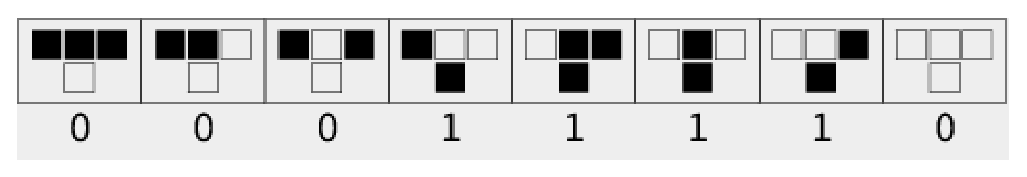
\includegraphics[width=\textwidth]{CA_Rule30.eps}
    \caption{\label{carule30} A schematic of rule 30}
\end{figure}

\begin{figure}
    \begin{minipage}[b]{0.49\textwidth}
        \centering
        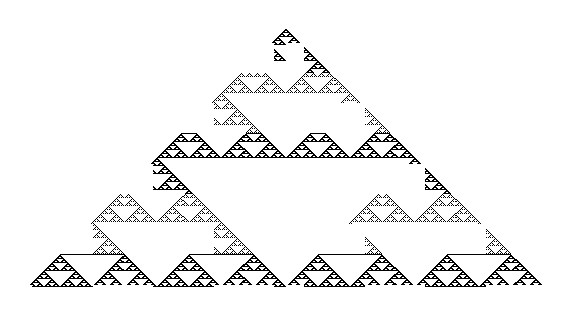
\includegraphics[width=\textwidth]{rule126.eps}
        \caption{\label{rule126} Rule 126}
    \end{minipage}
    \hspace{0.5cm}
    \begin{minipage}[b]{0.49\textwidth}
        \centering
        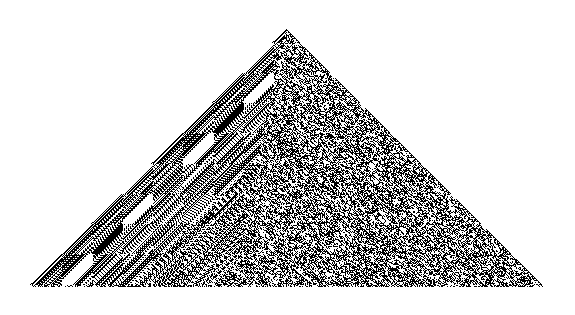
\includegraphics[width=\textwidth]{rule30.eps}
        \caption{\label{rule30} Rule 30}
    \end{minipage}
\end{figure}
